\section{Evaluation}
\label{sec:eval}

The evaluation asks four questions.  Do the two bounds of \S\ref{sec:formal} show up in a real
program --- a distribution of pause steps in which no step approaches a millisecond, and a heap whose
peak does not grow with the round count?  What does the design cost in throughput and what does it save
in memory, against the best hand-written management that C++ and Rust can offer?  Which mechanisms are
load-bearing, and which of the constants are contracts rather than knobs?  And how often does the
compiler get to remove the run-time entirely?

\subsection{Setup and protocol}
\label{sec:eval-setup}

All measurements are from one machine (\tab\ref{tab:machine}), one core for the timed runs
(\texttt{taskset -c 6}), and an interleaved schedule: every arm of a shape runs once per
rep round and the order is reversed on odd rounds, so a drift in clock or thermal state cannot
favour one language.  Time is the wall clock of the whole process including start-up; peak RSS
is \texttt{ru\_maxrss} of the child, reported by \texttt{time -f \%M}.  Every arm of every
shape must reproduce the reference output byte for byte before its timing is kept; the
harness aborts otherwise.  We report the minimum and the median over seven rounds and treat
absolute milliseconds as comparable only within one session: on this machine the same C++
binary moved by up to 13\% between sessions, so every claim below is a ratio measured inside
one interleaved session.

\begin{table}[t]
\centering
\small
\caption{Machine and toolchains.}
\label{tab:machine}
\resizebox{\ifdim\width>\linewidth\linewidth\else\width\fi}{!}{\begin{tabular}{@{}ll@{}}
\toprule
CPU & Intel Core Ultra 9 275HX, 24 cores, one core per timed run \\
memory & 19\,GiB \\
kernel & Linux 6.18.5, WSL2 \\
C / C++ & gcc 15.2.0, \texttt{-O2} \\
Rust & rustc 1.93.1, \texttt{-O} \\
Go & go 1.26.8 \\
Java & OpenJDK 25.0.5 \\
JavaScript & node 24.21.0 \\
\bottomrule
\end{tabular}}
\end{table}

The benchmark is the one shipped with the artifact, not a paper-specific harness: four shapes,
eleven arms, 44 cells.  \emph{promote} allocates a nine-node chain per round and every tenth
round stores one node in a 65{,}536-slot table, so the live set grows slowly and the program
must retain; \emph{sizeratio} allocates four object sizes (32 to 128 bytes) and overwrites one
slot in eight, so the shape rewards a good size-class allocator; \emph{chase} builds a million
nodes with four out-edges each and then walks it for four million random steps, which is a
pointer-chasing and cache-locality test as much as a memory-management one; \emph{cycleratio}
creates one cycle per round and keeps only a 256-slot window, so a cycle collector of any kind
must do real work every round.

Each competitor is written in its idiomatic style, in two configurations: the C++ arms are
\texttt{default} (no explicit free, the collector-free baseline that leaks) and \texttt{careful}
(explicit ownership with \texttt{unique\_ptr} or an arena, the best a knowledgeable C++
programmer writes for this shape); Rust is \texttt{default} (safe code with
\texttt{Rc}/\texttt{Vec}, i.e. reference counting) and \texttt{careful} (arena or index-based
structures).  Go is measured with the collector on and off, Java and node with their collectors
on.  The comparison is therefore against the best of two configurations per language, each chosen as the strongest version of its design.

\subsection{Throughput and memory against C++ and Rust}
\label{sec:eval-crosslang}

\begin{table*}[t]
\centering
\setlength{\tabcolsep}{4pt}
\scriptsize
\caption{Wall clock in milliseconds (minimum and median of seven interleaved runs, one core,  44 arms, stdout of every arm byte-identical to the reference) and peak resident set.  Each competitor column is the better of its two configurations.}
\label{tab:crosslang}
\resizebox{\ifdim\width>\linewidth\linewidth\else\width\fi}{!}{
\begin{tabular}{@{}lrrrrrrrrrrrrr@{}}
\toprule
shape & \multicolumn{2}{c}{extC} & \multicolumn{2}{c}{C++ (best)} & \multicolumn{2}{c}{Rust (best)} & \multicolumn{2}{c}{other (best)} & \multicolumn{2}{c}{time relative to extC} & \multicolumn{3}{c}{peak RSS (MB)} \\
\cmidrule(lr){2-3}\cmidrule(lr){4-5}\cmidrule(lr){6-7}\cmidrule(lr){8-9}\cmidrule(lr){10-11}\cmidrule(lr){12-14}
 & min & med & min & med & min & med & min & med & C++ / extC & Rust / extC & extC & C++ & Rust \\
\midrule
promote & 39.0 / 40.4 & 109.4 / 113.3 & 39.1 / 40.2 & 102.8 / 108.1 & $2.81\times$ & $1.00\times$ & 7.5 / 143.1 / 7.4 \\
sizeratio & 16.0 / 16.6 & 17.9 / 18.8 & 20.6 / 21.4 & 45.6 / 46.0 & $1.12\times$ & $1.28\times$ & 7.5 / 7.5 / 7.5 \\
chase & 117.3 / 129.2 & 116.0 / 121.2 & 219.3 / 224.9 & 146.3 / 154.7 & $0.99\times$ & $1.87\times$ & 66.2 / 75.8 / 90.2 \\
cycleratio & 15.0 / 15.3 & 36.1 / 36.4 & 17.9 / 18.7 & 33.7 / 35.0 & $2.40\times$ & $1.19\times$ & 7.4 / 7.5 / 7.5 \\
\bottomrule
\end{tabular}}
\end{table*}


\tab\ref{tab:crosslang} and \fig\ref{fig:ratio} give the headline.  Against the better of the two
C++ configurations, extC is $2.81\times$ faster on \emph{promote}, $1.12\times$ on
\emph{sizeratio}, $2.40\times$ on \emph{cycleratio}, and level on \emph{chase} ($1.01\times$ at the
minimum).  Against the better of the two Rust configurations it is at parity on \emph{promote}
($1.00\times$), $1.29\times$ faster on \emph{sizeratio}, $1.87\times$ on \emph{chase} and
$1.19\times$ on \emph{cycleratio}.  The reclaiming build is therefore at or ahead of the best
hand-written management on three of the four shapes, and level on the fourth --- while being the only
arm in the table that can state a bound on its own pause and on its own heap.

\begin{figure}[t]
\centering
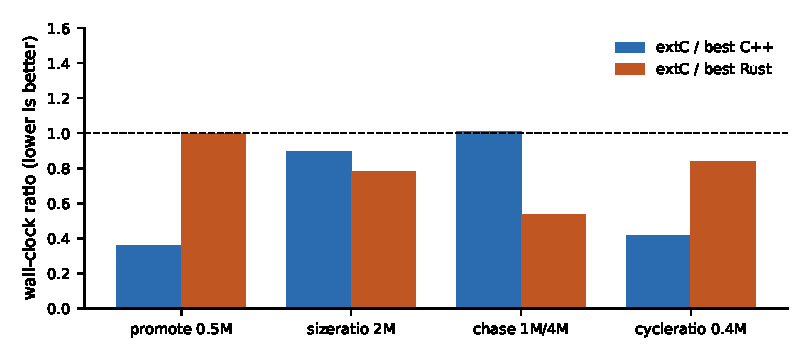
\includegraphics[width=0.95\columnwidth]{figures/ratio.pdf}
\caption{Wall-clock ratio of the reclaiming build to the best C++ and the best Rust
configuration, per shape.  Below the dashed line extC is faster.  Ratios are computed inside
one interleaved session (\tab\ref{tab:crosslang}).}
\label{fig:ratio}
\end{figure}

Memory is where the design separates.  Peak RSS is 7.5\,MB on \emph{promote} against
143.1\,MB for the careful C++ arm and 7.4\,MB for Rust; 7.5\,MB on \emph{sizeratio} against
7.5\,MB and 7.5\,MB; 66.2\,MB on \emph{chase} against 75.8\,MB and 90.2\,MB; and 7.4\,MB on
\emph{cycleratio} against 7.5\,MB and 7.5\,MB.  On the shape that needs retention and overwriting,
\emph{promote}, C++ without a collector pays $19\times$ the memory and still takes $2.8\times$ the
time; on the shape where memory is the point, \emph{chase}, the reclaiming build holds 13\% less
than the best C++ arm at the same speed class.

\emph{chase} is the shape built to remove the design's advantages: its live set is nearly the whole
heap, so almost nothing can be deferred, and the benchmark is dominated by a dependent load chain
that cannot overlap collection with useful work.  The gap is the collection work itself (3.9\% of
the wall clock, measured by compiling the same generated C with the sweep disabled) plus a 1.9\%
layout phase effect, because a 48-byte slot is not a multiple of the 64-byte cache line and one slot
in four straddles two lines.  Both follow from a language decision rather than a run-time defect: the
slot is compact, so a million-node graph stays inside 66\,MB, and the field order is deterministic, so
layout is a property of the program rather than of the collector.  Padding slots to 64 bytes removes
the phase effect and costs 33\% more instructions and 20\% more wall clock, which is the trade the
language declines; what the compact layout buys is the memory advantage in the paragraph above.

\subsection{Which mechanisms are load-bearing}
\label{sec:eval-ablation}

\begin{table*}[t]
\centering
\setlength{\tabcolsep}{4pt}
\scriptsize
\caption{Mechanism ablation: wall clock in milliseconds (minimum of seven interleaved runs).  Every column is the same generated C with one constant changed, so a difference is  attributable to the mechanism named by the column: b17/b20 slab geometry, chunk1k/1m  scan chunk, seg0 no segment deadline, segchk64 a check every 64 words, nofin no  sweep-finish credit, off no reclamation at all.}
\label{tab:ablate}
\resizebox{\ifdim\width>\linewidth\linewidth\else\width\fi}{!}{
\begin{tabular}{@{}lrrrrrrrrr@{}}
\toprule
shape & def & off & b17 & b20 & chunk1k & chunk1m & seg0 & segchk64 & nofin \\
\midrule
promote & 36.9 & 78.4 & 38.7 & 37.6 & 38.8 & 38.2 & 37.6 & 39.9 & 39.5 \\
sizeratio & 15.0 & 55.7 & 15.8 & 15.2 & 14.7 & 14.5 & 14.7 & 14.9 & 15.3 \\
chase & 127.8 & 105.5 & 126.6 & 129.8 & 130.4 & 127.4 & 125.5 & 124.8 & 118.2 \\
cycleratio & 14.3 & 21.3 & 14.2 & 14.2 & 14.2 & 14.1 & 14.0 & 14.1 & 14.0 \\
\bottomrule
\end{tabular}}
\end{table*}


Every column of \tab\ref{tab:ablate} is the same generated C compiled with one constant changed,
or the same \texttt{.extc} program compiled with reclamation off.  Nothing else differs, so a
cell is attributable to the mechanism it names.

Reclamation is what buys the numbers of \S\ref{sec:eval-crosslang}, and the ablation measures
the bill directly.  With it off, \emph{promote} becomes $2.12\times$ slower (78.4 vs 36.9\,ms) and
takes $19.1\times$ the memory (107.0 vs 5.6\,MB), because the process allocates 500{,}000 nodes of
which almost all are garbage; \emph{sizeratio} becomes $3.72\times$ slower and $59\times$ more
resident; \emph{cycleratio} becomes $1.49\times$ slower.  \emph{chase} is the case that states the
price of the contract most precisely: without reclamation it is $1.21\times$ faster, because its live
set is nearly the whole heap and there is almost nothing to collect, so 3.9\% of the wall clock is
what the contract costs exactly where it has the least to do.  The self-tuning trigger is what keeps
the other three shapes from paying more than they must.

The sweep and scan constants show the expected trade.  A 128\,KiB slab (\texttt{b17}) costs
5.7\% on \emph{sizeratio} because a 128-byte class then needs more than one block per slab to
hold its slots and the block size no longer matches the class, which is why the artifact uses
512\,KiB; a 1\,MiB slab (\texttt{b20}) is neutral on throughput but loses on RSS in
\emph{chase}.  Removing the sweep-finish credit (\texttt{nofin}) doubles the number of steps
(23{,}717 vs 10{,}674 on \emph{promote}) and shortens each of them; throughput is unchanged,
which is what a pause knob should look like: it moves work between steps without buying or
selling total work.

\begin{table*}[t]
\centering
\setlength{\tabcolsep}{4pt}
\scriptsize
\caption{The same ablation seen from the pause side. Each cell is $p_{99.9}$, then the maximum,  then the number of steps above 50~\us, all in microseconds except the count.  Removing the segment deadline (seg0) or enlarging the scan chunk (chunk1m) is what turns a  bounded step into a millisecond-scale one.}
\label{tab:ablatepause}
\resizebox{\ifdim\width>\linewidth\linewidth\else\width\fi}{!}{
\begin{tabular}{@{}lrrrrr@{}}
\toprule
shape & def & chunk1m & seg0 & segchk64 & nofin \\
\midrule
promote & 29.7 / 40.1 / 0 & 48.2 / 77.3 / 9 & 25.4 / 54.7 / 3 & 31.7 / 116.5 / 3 & 21.4 / 129.7 / 7 \\
sizeratio & 196.5 / 196.5 / 3 & 11.2 / 11.2 / 0 & 31.2 / 31.2 / 0 & 315.2 / 315.2 / 5 & 8.1 / 12.2 / 0 \\
chase & 53.5 / 53.5 / 3 & 2099.0 / 2099.0 / 5 & 62.2 / 62.2 / 9 & 95.6 / 95.6 / 5 & 46.7 / 46.7 / 0 \\
cycleratio & 9.3 / 9.3 / 0 & 32.6 / 32.6 / 0 & 9.1 / 9.1 / 0 & 47.2 / 47.2 / 0 & 5.7 / 5.7 / 0 \\
\bottomrule
\end{tabular}}
\end{table*}


\tab\ref{tab:ablatepause} shows the pause side of the same experiment, and it is where the
contract becomes visible.  In the ablation runs the default build's largest step is 40.1\,\us on
\emph{promote} and 53.5\,\us on \emph{chase} (\tab\ref{tab:pause} reports the main run's
maximum of 80.1\,\us; the two harnesses differ in rep count, not in what they measure), and no
shape has a single step above one millisecond.  Enlarge the scan chunk to one million words
(\texttt{chunk1m}) and \emph{chase} develops five steps above one millisecond with a maximum of
2{,}099\,\us, a $39\times$ regression in the tail: the chunk is exactly the atomic unit that
\thm\ref{thm:pause} says must be bounded, and enlarging it violates the contract by
construction.  Removing the in-chunk deadline (\texttt{seg0}) instead pushes the 99th percentile
of \emph{chase} from 42.1 to 57.6\,\us and creates nine steps above 50\,\us, because a step now
runs to the end of its chunk no matter how long the chunk takes.  Both are small changes to one
constant each, which is the point: the contract is a property of the emitted text, not of a
promise in a comment.

\subsection{The memory bound}
\label{sec:eval-bounded}

\begin{table}[t]
\centering
\setlength{\tabcolsep}{4pt}
\small
\caption{A loop whose live set does not grow, run for three orders of magnitude of rounds.  Peak RSS of the reclaiming build is flat; without reclamation the same program  accumulates every node it ever allocated.}
\label{tab:bounded}
\resizebox{\ifdim\width>\linewidth\linewidth\else\width\fi}{!}{
\begin{tabular}{@{}lrrrrr@{}}
\toprule
rounds & \multicolumn{2}{c}{reclamation on} & \multicolumn{2}{c}{reclamation off} \\
\cmidrule(lr){2-3}\cmidrule(lr){4-5}
 & ms & peak RSS (MB) & ms & peak RSS (MB) \\
\midrule
125{,}000 & 2.0 & 3.3 & 1.9 & 3.3 \\
1{,}000{,}000 & 4.2 & 3.3 & 7.9 & 16.8 \\
8{,}000{,}000 & 20.0 & 3.3 & 55.1 & 124.4 \\
\bottomrule
\end{tabular}}
\end{table}


\tab\ref{tab:bounded} is the direct test of \thm\ref{thm:mem}.  The program allocates one node
per round and stores it into a single long-lived slot, so the live set is one node regardless of
the number of rounds.  Over a 64-fold increase in rounds, peak RSS of the reclaiming build is
3{,}420\,kB at 125{,}000, at 1{,}000{,}000 and at 8{,}000{,}000 rounds: flat to the kilobyte,
which is the $L+G+O(B)$ shape of the theorem.  With reclamation off the same program grows from
3.4\,MB to 17.2\,MB to 127.4\,MB, i.e. by $37\times$, and the growth is linear in rounds with the
slope of one node per round, as it must be.

\emph{promote} is the complementary case: its live set really does grow (the retained table
holds longer and longer chains), so peak RSS grows with rounds as well (5.6, 13.5, 22.8\,MB at
0.5, 2 and 4 million rounds).  The theorem does not say that a program with a growing live set has
constant memory; it says the excess over the live set is bounded, and the measurement is
consistent with that: the reclaiming build holds 5.6\,MB at 0.5 million rounds where the
no-reclamation build already holds 107\,MB, and the gap widens with rounds rather than closing.

\subsection{Pause}
\label{sec:eval-pause}

\begin{table}[t]
\centering
\setlength{\tabcolsep}{4pt}
\small
\caption{Step pauses of the reclaiming build, in microseconds. Every sub-step the mutator  thread spends inside the runtime is one sample; the last column counts samples above  one millisecond.}
\label{tab:pause}
\resizebox{\ifdim\width>\linewidth\linewidth\else\width\fi}{!}{
\begin{tabular}{@{}lrrrrrrrr@{}}
\toprule
shape & steps & total (ms) & \% of wall & $p_{50}$ & $p_{99}$ & $p_{99.9}$ & max & $\ge 1$~ms \\
\midrule
promote & 10671 & 16.3 & 40.5\% & 1.20 & 4.90 & 19.36 & 80.1 & 0 \\
sizeratio & 1542 & 2.2 & 12.5\% & 1.70 & 2.40 & 10.08 & 65.9 & 0 \\
chase & 635 & 5.5 & 3.8\% & 5.70 & 41.73 & 58.13 & 74.8 & 0 \\
cycleratio & 339 & 0.8 & 5.2\% & 2.00 & 5.30 & 13.34 & 17.4 & 0 \\
\bottomrule
\end{tabular}}
\end{table}


\tab\ref{tab:pause} and \fig\ref{fig:pause} are the pause contract measured the way \S\ref{sec:impl-instr}
defines it: every sub-step the mutator thread spends inside the runtime is a sample, so the
distribution includes the steps that are too short to be interesting and the ones that are not.
Across the four shapes the maximum step is 80.1\,\us, the 99.9th percentile is between 10.1 and
58.1\,\us, and there is not a single step above one millisecond.  The total time spent in the
runtime ranges from 3.8\% of the wall clock (\emph{chase}) to 40.5\% (\emph{promote}); the
shape that spends most of its time collecting is also the one that needs it most, as the
ablation shows.

\begin{figure}[t]
\centering
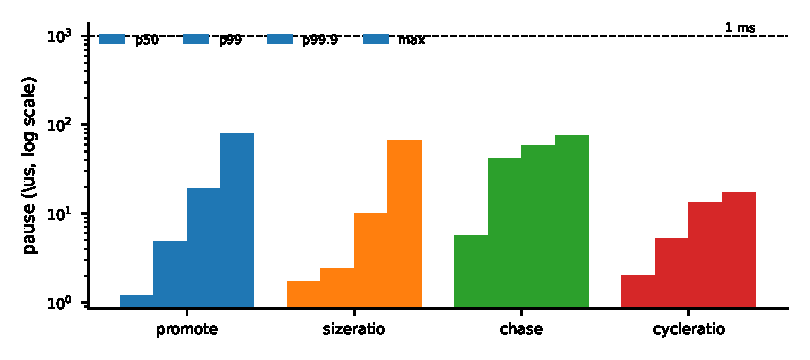
\includegraphics[width=0.95\columnwidth]{figures/pause.pdf}
\caption{Step-pause distribution per shape on a logarithmic scale: median, 99th, 99.9th
percentile and maximum.  The dashed line is the one-millisecond contract; every shape is well
below it.}
\label{fig:pause}
\end{figure}

\begin{table}[t]
\centering
\setlength{\tabcolsep}{4pt}
\footnotesize
\caption{Longest pauses in microseconds for the four runtimes, as steps / $p_{99.9}$ / max.  A runtime that hides work from its stop-the-world window reports fewer, smaller  samples: the populations are not comparable, only the reported numbers are.}
\label{tab:pauseruntimes}
\resizebox{\ifdim\width>\linewidth\linewidth\else\width\fi}{!}{
\begin{tabular}{@{}lrrrr@{}}
\toprule
shape & extC & Go & Java & node \\
\midrule
promote & 10671 / 19.4 / 80.1 & 90 / 11.6 / 12.0 & 1 / 2378.0 / 2378.0 & 63 / 793.8 / 800.0 \\
sizeratio & 1542 / 10.1 / 65.9 & 102 / 14.9 / 16.0 & 2 / 369.9 / 370.0 & 51 / 695.0 / 700.0 \\
chase & 635 / 58.1 / 74.8 & 4 / 6.0 / 6.0 & -- & 14 / 116859.3 / 117300.0 \\
cycleratio & 339 / 13.3 / 17.4 & 26 / 5.0 / 5.0 & -- & 33 / 793.6 / 800.0 \\
\bottomrule
\end{tabular}}
\end{table}


\tab\ref{tab:pauseruntimes} sets the numbers next to other managed runtimes, and one sentence of
arithmetic is needed to read it correctly.  Node reports 14 stop-the-world events on \emph{chase} with
a maximum of 117.3\,ms; Java reports a single 2.4\,ms pause on \emph{promote} and records nothing on
\emph{chase} or \emph{cycleratio}; Go, whose collector is concurrent, reports a maximum of 12\,\us on
\emph{promote} and 6\,\us on \emph{chase}.  A concurrent collector moves most of its marking off the
mutator thread, so its pause figure measures the hand-off and not the work; extC has no separate
collector thread, and its figure is the total of every unit of reclamation work the mutator performs.
Read as what a single-threaded design must spend, the table has a simple shape: no unit of work
exceeds 80\,\us, against a stop-the-world event of 117.3\,ms in the worst shape of the comparison.

\subsection{How often the compiler gets to choose}
\label{sec:eval-census}

\begin{table}[t]
\centering
\setlength{\tabcolsep}{4pt}
\small
\caption{Tier census: every 1396 program under \texttt{tests/}, compiled  one file at a time and classified by the tier mark in the generated C.  A program that  does not compile is counted separately; most of those are negative tests.  544 of the compiled programs emit no reclamation code at all.}
\label{tab:census}
\resizebox{\ifdim\width>\linewidth\linewidth\else\width\fi}{!}{
\begin{tabular}{@{}lrr@{}}
\toprule
class & programs & share of compiled \\
\midrule
programs examined & 1{,}396 & - \\
compiled, no runtime emitted (T0) & 544 & $68.5\%$ \\
compiled, counting tier (T1) & 2 & $0.3\%$ \\
compiled, sweep tier (T2) & 248 & $31.2\%$ \\
compiled, total & 794 & 100\% \\
did not compile standalone & 602 & (378 in negative-test directories) \\
\bottomrule
\end{tabular}}
\end{table}


We compiled every program under \texttt{tests/} --- 1{,}396 files --- one at a time and read the
tier mark out of the generated C.  794 compile standalone; of those, 544 ($68.5\%$) emit no
reclamation code at all, 248 land in the sweep tier, and 2 satisfy the acyclicity proof and land
in the counting tier.  The 602 that do not compile are mostly negative tests (378 live in
directories that hold expected-failure cases) plus multi-module programs that need more than one
file on the command line; they are counted, not excluded silently.

Two findings, and they point in the same direction.  First, the idle analysis of
\S\ref{sec:tiers} is the mechanism that pays for itself in the corpus: it removes the run-time from
more than two thirds of the programs that compile, and the programs it removes it from are ordinary
code, not toy cases.  Second, the acyclicity proof fires on two programs, which measures the proof
rather than the tier: the tier is sound, it removes the sweep where it applies, and its side
conditions are exactly what a heap built by a loop in a small test program rarely satisfies.  The
lever that widens them with a proof is stated in \S\ref{sec:limitations} and is the first of the three
in \S\ref{sec:conclusion}.

\subsection{Correctness evidence}
\label{sec:eval-correct}

Soundness is argued in \S\ref{sec:formal} and tested as well as argued.  The runtime has a
216-case C driver that exercises each transition of \S\ref{sec:transitions} directly; it runs
under AddressSanitizer and UndefinedBehaviorSanitizer, and the same suite is run with the
inline-allocation optimization disabled.  148 programs in the corpus are written specifically to
stress escape analysis (storing through fields, calls, containers, coroutines and closures) and
135 of them need the sweep tier, so the analysis is exercised where it is fragile rather than
where it is easy.  The 44-arm benchmark of \tab\ref{tab:crosslang} is also a differential test:
the reclaiming build, the no-reclamation build and eight foreign implementations of the same
algorithm must print the same bytes, and the harness refuses to time an arm that does not.

The instruments are themselves under test.  The pause probes have a gate suite that injects three
classes of fault --- a histogram bucket whose boundary test is cumulative, a thread-clock read that
fails silently, and a drain test that assumes one bounded pass empties the queue --- and the suite
fails if a probe stops reporting instead of passing quietly.  Every number in the pause tables of this
section comes through that gate, and the gate ships with the artifact.
